\subsection{Collision Detection for Rotated Objects}
The user should be able to select the object by clicking inside of the hitbox, even when the object is rotated.
This gave an issue when rotating an object the hitbox did not follow and to click on the object you had to click inside the misplaced hitbox.

The reason for this was that when the object was created the hitbox was set but never changed after rotating the object.
Therefore, a change was made to the hitbox property such that the top left corner of the hitbox was set to the minimum x and y value of an objects coordinates.

To find the new points of the rotated object we used the rotation matrix to rotate the current corners of the object.
As seen in \lstref{lst:changeHitbox} the minimum x and y values of these corners are then found, and used to find the top left corner of the hitbox.
Once this corner has been found, the width and height can be calculated by using the corner and the center of the object.

In \figref{figure:hitbox} the hitbox can be seen around the hitbox both when rotated and not rotated.

\begin{lstlisting}[caption={Method to change the hitbox},label=lst:changeHitbox]
protected void changeHitbox(){
	FloatPoint one = rotationMatrix( -(getWidth()/2), -(getHeight()/2));
	FloatPoint two = rotationMatrix((getWidth()/2), -(getHeight()/2));
	FloatPoint three = rotationMatrix((getWidth()/2), (getHeight()/2));
	FloatPoint four = rotationMatrix( -(getWidth()/2), (getHeight()/2));
	
	hitboxTopLeft = new FloatPoint(
	    findMin(one.x, two.x, three.x, four.x),
	    findMin(one.y, two.y, three.y, four.y));
	hitboxWidth = (getCenter().x - hitboxTopLeft.x)*2;
	hitboxHeigth = (getCenter().y - hitboxTopLeft.y)*2;
}
\end{lstlisting}



\begin{figure}[h]
	\centering
	%---- linebreak	
	\begin{subfigure}[b]{0.45\textwidth}
		\centering
		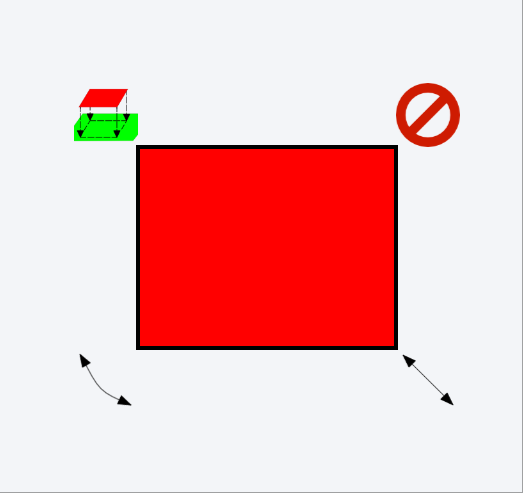
\includegraphics[scale = 0.3]{sprint1/rectangle}
		\caption{Hitbox for standard rectangle}
		\label{figure:hitbox-rectangle}
	\end{subfigure}
	\qquad
	\begin{subfigure}[b]{0.45\textwidth}
		\centering
		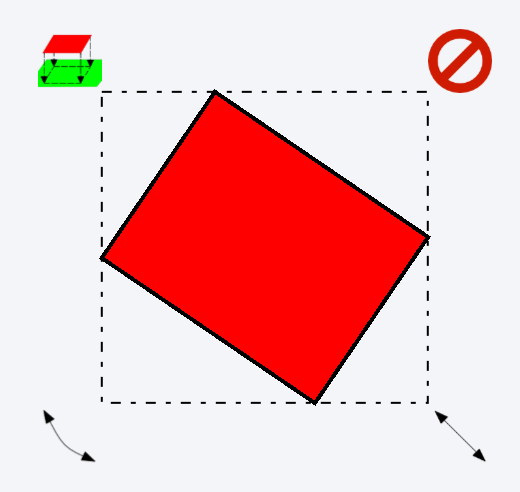
\includegraphics[scale = 0.3]{sprint1/rectangle-rotated}
		\caption{Hitbox for a rotated rectangle.}
		\label{figure:hitbox-rotated-rectangle}
	\end{subfigure}
	\caption{The different hitboxes.}
	\label{figure:hitbox}
\end{figure}

A new issue that emerged was that the collision detection for the object was now larger than the object.
When an object was behind a rotated object, and the user clicked the in the top left corner of the hitbox, the rotated object would be selected instead of the object behind.
To resolve this issue, an implementation was done to give a precise collision detection on the object, which will be described below.

\subsubsection{Precise Collision Detection for Rotated Rectangles}
To understand the mathematics behind the precise collision detection for rotated rectangles, an illustration of the problem can be seen in \figref{figure:rectangle-collision}.

\begin{figure}[h]
	\centering
	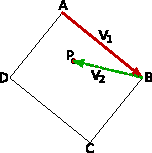
\includegraphics[scale=2]{sprint1/rectangle-collision}
	\caption{Vectors showing a right rotation.}
	\label{figure:rectangle-collision}
\end{figure}

The idea behind the mathematical formula is to see whether the vector to the point is a right rotation of all the rectangle's sides.
To determine this we compare the slope of the vectors.
The formula to determine a right rotation is:
\begin{equation}
	\frac{B_x-A_x}{B_y-A_y} \geq \frac{P_x-B_x}{P_y-B_y}
\end{equation}

The formula is changed to avoid divide by zero errors, and is therefore changed to the following equation:
\begin{equation}
	(B_x-A_x)*(P_y-B_y) \geq (P_x-B_x)*(B_y-A_y)
\end{equation} 

\subsubsection{Precise Collision Detection for Rotated Ellipses}


\subsubsection{Precise Collision Detection for Rotated Lines}
The last collision issue was a precise implementation to click on a line.
We discussed how to click on a line and agreed that the click is allowed to be slightly off the line, since it otherwise was hard to click on.
An idea was to calculate the distance from a point to the line and add a "jitter" range which determined the range of how close the point had to be to the line.

To find this distance we used the formula for finding the area of a triangle, since the three points, clicked point, start point and end point of the line, formed a triangle.
The distance is determined by the height of the triangle, from the base to the clicked point as seen in \figref{figure:line-collision}.
\begin{figure}[h]
	\centering
	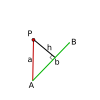
\includegraphics[scale=2]{sprint1/line-collision}
	\caption{Drawing showing the idea behind the mathematical formula.}
	\label{figure:line-collision}
\end{figure}

There are two formulas for finding the area of a triangle, as seen in \eqref{eq:area1} and \eqref{eq:area2}.

\begin{equation}\label{eq:area1}
	A = \frac{1}{2}*h*b
\end{equation}

\begin{equation}\label{eq:area2}
	A =  \frac{1}{2}*|\vec{a} \times \vec{b}|
\end{equation}

We can combined these two formulas since we are not interested in the area but the height $h$.
Once combined, we can isolate the height $h$ and find a final equation for the height, as seen in \eqref{eq:isolated-h}.
\begin{equation}\label{eq:isolated-h}
\begin{aligned}
	\frac{1}{2}*h*b &=  \frac{1}{2}*|\vec{a} \times \vec{b}|\\
	& \Downarrow \\
	h &=  \frac{|\vec{a} \times \vec{b}|}{b}
\end{aligned}
\end{equation}

Another note to mention, is that the length of the vector $\vec{b}$ is the same as the base $b$.

\begin{equation*}
	|\vec{b}| = b
\end{equation*}

Since \eqref{eq:isolated-h} is based on given vectors and lengths, and the variables given in the program are coordinates, we have to change the formula to calculate the vectors and lengths from the coordinates.
As can be seen in \eqref{eq:cross-product}, the vector $\vec{a}$ is equal to the difference in the clicked point $P$ and the start point $A$.
\begin{equation}\label{eq:cross-product}
	|\vec{a} \times \vec{b}| = 
	\begin{bmatrix}
		P_x-A_x \\
		P_y-A_y
	\end{bmatrix}
	\times
	\begin{bmatrix}
		B_x-A_x \\
		B_y-A_y
	\end{bmatrix}
\end{equation}

From \eqref{eq:cross-product}, we can see how the cross product of the two vectors is determined, given the three coordinates.
We can now replace that with the cross product in \eqref{eq:isolate-h}, and add the equation for finding the length of the vector $\vec{b}$ in the denominator, as seen in \eqref{eq:final-line-formula}.
By expanding the brackets in the numerator, we get a final equation for finding the distance from a point to a line that goes through two points.

\begin{equation}\label{eq:final-line-formula}
\begin{aligned}
	h &= \frac{|\vec{a} \times \vec{b}|}{|\vec{b}|}\\
	  &= \frac{|(P_x-A_x)(B_y-A_y)-(P_y-A-y)(B_x-A_x)|}{\sqrt{b_x^2+b_y^2}}\\
	  &= \frac{|P_xB_y-P_xA_y-A_xB_y-P_yB_x+P_yA_x+A_yB_x|}{\sqrt{b_x^2+b_y^2}}
\end{aligned}
\end{equation}

Since the equation finds the distance from the clicked point and a line that goes through two known points, we have to limit the line so it does not go passed the two points.
To do this limitation, we use the hitbox of the line so that the click also has to be inside of the hitbox.








